\documentclass[aspectratio=169]{beamer}

\usepackage[UTF8, heading]{ctex} % 中文支持
\usepackage{color}
\usepackage{amsmath}
\usepackage{svg}          % 插入 svg 矢量图
\usepackage{tikz}         % 绘图
\usepackage{subcaption}   % 创建子图
\usepackage{minted}       % 代码高亮
\usepackage[ruled,linesnumbered]{algorithm2e}  % 伪代码
\usepackage{lmodern}      % 消除 warning
\usepackage{ncepu-beamer} % 应用主题

% 指定 inkscape 路径(inkscape 用于处理 svg 矢量图)
\setsvg{inkscapeexe={"C:/Program Files/Inkscape/bin/inkscape.com"}}
% 设置 svg 文字随图片缩放
\svgsetup{inkscapelatex=false}
% NOTE: draw.io 中的文本需要关闭自动换行和格式化文本

% 使用 tikz 绘制大括号
\usetikzlibrary{decorations.pathreplacing}
% 使用 tikz 绘制流程图
\usetikzlibrary{shapes.geometric, arrows}
\tikzstyle{startstop} = [rectangle, rounded corners, minimum width=1.5cm, minimum height=0.75cm,text centered, draw=black, fill=red!30]
\tikzstyle{io} = [trapezium, trapezium left angle=70, trapezium right angle=110, minimum width=1.5cm, minimum height=0.75cm, text centered, draw=black, fill=blue!30]
\tikzstyle{process} = [rectangle, minimum width=1.5cm, minimum height=0.75cm, text centered, draw=black, fill=orange!30]
\tikzstyle{decision} = [diamond, minimum width=1.5cm, minimum height=0.75cm, text centered, draw=black, fill=green!30]
\tikzstyle{arrow} = [thick,->,>=stealth]

% 输入信息
\title{基于DRL的动态租用实例任务调度}
\author{刘肇泽}
\institute{控制与计算机工程学院}
\date{\today}

\begin{document}

\begin{frame}[noframenumbering]

    \titlepage

\end{frame}

\begin{frame}{目录}

    \centering
    \begin{minipage}{0.8\textwidth}
        \tableofcontents
    \end{minipage}

\end{frame}

\begin{frame}{摘要}

    与 Cost-Aware 的不同之处:

    \begin{enumerate}
        \item 引入了 On Demand 和 Spot 两种计费规则的实例
        \item 引入了 Moldable 和 Rigid 两种任务类型
        \item 引入了任务的挂起、恢复和跨区域调度
    \end{enumerate}

\end{frame}

\section{数学模型}

\begin{frame}

    \centering
    使用 $T$ 表示时间段, $t$ 表示时刻.

\end{frame}

\subsection{实例建模}

\begin{frame}{实例 (Instance) 的数学模型}

    \begin{columns}

        \column{0.5\textwidth}

        固有属性:

        \begin{itemize}
            \item $I_c$ 实例的计算核心数
            \item $I_m$ 实例的内存大小
            \item $I_r$ 实例所在区域
            \item $I_b$ 实例的计费类型 (On Demand/Spot)
            \item $v_s$ 实例中任务挂起 (suspend) 速度
            \item $v_r$ 实例中任务恢复 (resume) 速度
        \end{itemize}

        \column{0.5\textwidth}

        状态属性:

        \begin{itemize}
            \item $T_r$ 实例的剩余租期 (remain time)
            \item $t_i$ 实例空闲的时刻 (idle time)
        \end{itemize}

    \end{columns}

    \vspace{1em}

    计费类型:

    \begin{itemize}
        \item On Demand: 每小时价格固定
        \item Spot: 每小时价格随市场波动
    \end{itemize}

\end{frame}


\subsection{任务建模}

\begin{frame}{任务 (Job) 的数学模型}

    \begin{columns}

        \column{0.5\textwidth}

        固有属性:

        \begin{itemize}
            \item $J_c$ 任务需要的计算核心数
            \item $J_m$ 任务需要的内存大小
            \item $J_t$ 任务的类型 (Moldable/Rigid)
        \end{itemize}

        \column{0.5\textwidth}

        状态属性:

        \begin{itemize}
            \item $J_l$ 任务长度(小时)
            \item $t_a$ 任务到达时刻 (arrival time)
            \item $J_r$ 任务上一次执行所在的区域
        \end{itemize}

    \end{columns}

\end{frame}

\begin{frame}{Downey 加速模型}

    并行度 (parallelism) 具有均值 $A$ 和标准差 $\sigma$ 两个参数.

    将 $0 \leqslant \sigma \leqslant 1$ 的模型称为Low variance model, 将 $\sigma > 1$ 的模型称为High variance model.

    \begin{columns}

        \column{0.5\textwidth}

        \begin{figure}
            \centering
            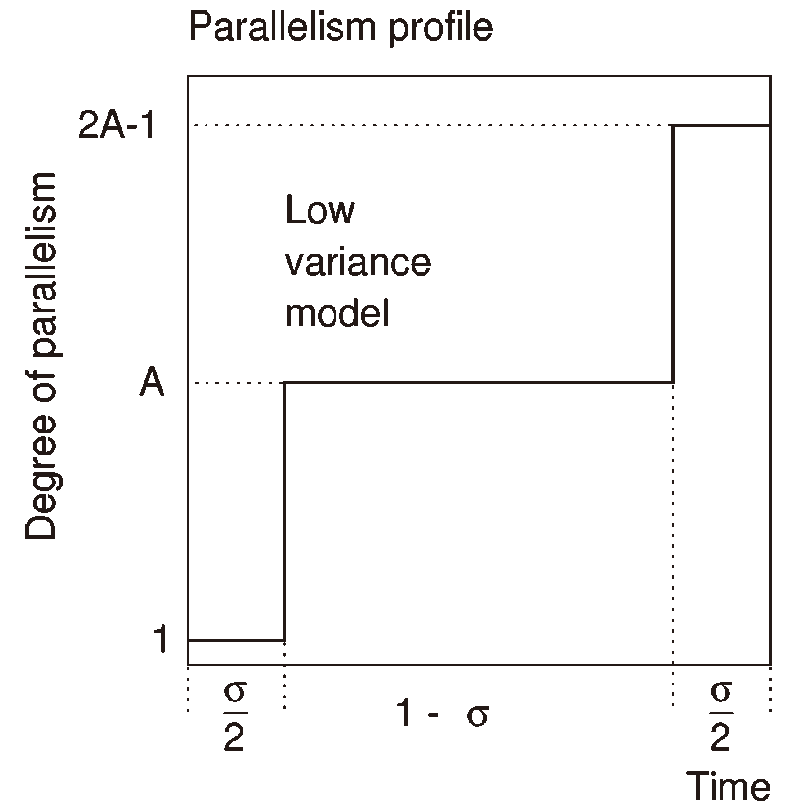
\includegraphics[scale=0.15]{pics/low_variance_model.png}
            \caption{Low variance model}
        \end{figure}

        \column{0.5\textwidth}

        \begin{figure}
            \centering
            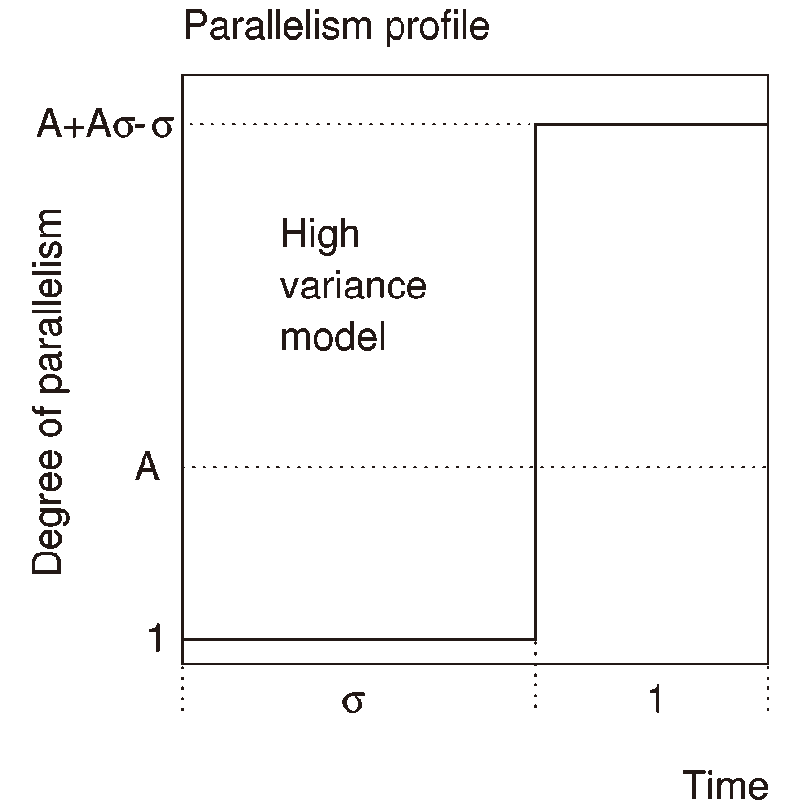
\includegraphics[scale=0.15]{pics/high_variance_model.png}
            \caption{High variance model}
        \end{figure}

    \end{columns}

\end{frame}

\begin{frame}{Downey 加速模型}{加速系数 $SU(n)$ 的计算}

    \begin{columns}

        \column{0.6\textwidth}

        当 $0 \leqslant \sigma \leqslant 1$ 时:

        \begin{equation*}
            SU(n)= \begin{cases}
                \frac{A n}{A + \sigma(n-1) / 2},                 & 1 \leqslant n \leqslant A, \\
                \frac{A n}{\sigma(A-1 / 2) + n(1 - \sigma / 2)}, & A < n \leqslant 2 A-1,     \\
                A,                                               & n > 2A - 1 .
            \end{cases}
        \end{equation*}

        当 $\sigma > 1$ 时:

        \begin{equation*}
            SU(n)= \begin{cases}
                \frac{n A(\sigma + 1)}{A + A \sigma - \sigma + n \sigma}, & 1 \leqslant n \leqslant A + A \sigma - \sigma, \\
                A,                                                        & n > A + A \sigma - \sigma .
            \end{cases}
        \end{equation*}

        其中 $n$ 为计算核心数.

        \column{0.4\textwidth}

        \begin{figure}
            \centering
            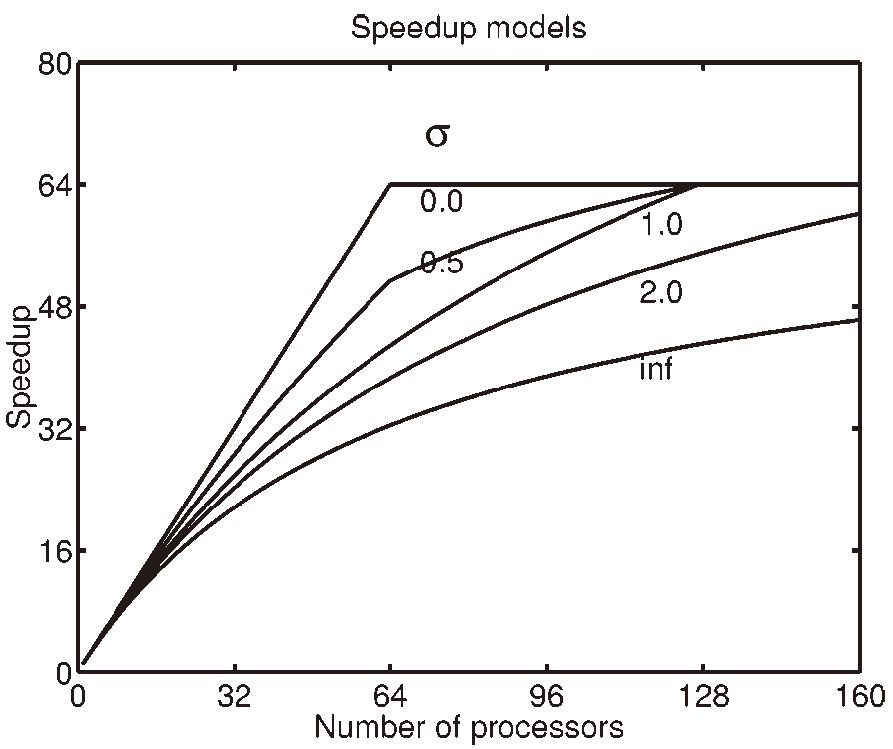
\includegraphics[scale=0.17]{pics/speedup_curve.png}
            \caption{Speedup curves for a range of values of $\sigma$ when $A = 64$}
        \end{figure}
    \end{columns}
\end{frame}

\begin{frame}[fragile]{任务类型 $J_t$ 与实际执行时间 $T^e$}{Moldable/Rigid}

    任务类型 $J_t$ 影响任务实际执行时间 $T^e$ 的计算.

    \centering
    \begin{minipage}{0.7\textwidth}
        \IncMargin{1.5em}
        \begin{algorithm}[H]
            \SetAlgoLined
            \caption{计算任务实际执行时间 $T^e$}
            \If{$J_t =$ Moldable}{$T^e = J_l \cdot \frac{SU(J_c)}{SU(I_c)}$\;}
            \If{$J_t =$ Rigid}{\eIf{$J_c \leqslant I_c$}{$T^e = J_l$\;}{任务调度失败\;}}
        \end{algorithm}
        \DecMargin{1.5em}
    \end{minipage}

\end{frame}

\begin{frame}{挂起时间 $T_w$ 与恢复时间 $T_l$}

    当正在执行任务的实例到期时, 任务需要挂起到硬盘, 该操作需要的时间为:

    \begin{equation*}
        T_w = \frac{J_m}{v_w}
    \end{equation*}

    当任务首次在实例中运行或从挂起状态恢复时, 任务需要加载到内存, 该操作需要的时间为:

    \begin{equation*}
        T_l = \begin{cases}
            \dfrac{J_m}{v_l},          & J_r = None \, \text{or} \, J_r = I_r, \\
            2 \times \dfrac{J_m}{v_l}, & \text{otherwise}.
        \end{cases}
    \end{equation*}

\end{frame}


\subsection{任务调度流程建模}

\begin{frame}{任务调度流程}

    \scriptsize
    \begin{tikzpicture}[node distance=1.5cm]
        \node (start) [startstop] {Start};
        \node (in) [io, below of=start] {Input: 当前任务 $J$ 所选实例 $I$};
        \node (memory check) [decision, below of=in, yshift=-0.5cm] {$J_m \leqslant I_m$};
        \node (core check) [decision, right of=memory check, xshift=2cm, align=center] {$J_t = Rigid$\\\&\\$J_c > I_c$};
        \node (out of memory) [process, below of=memory check, yshift=-1cm, align=center] {任务调度失败\\$reward = -100$};
        \node (insufficient cores) [process, below of=core check, yshift=-1cm, align=center] {任务调度失败\\$reward = -100$};
        \node (calculate) [process, right of=core check, xshift=2.5cm, align=center] {计算实际执行时间 $T^e$\\挂起时间 $T^s$\\恢复时间 $T^r$};
        \node (update) [process, right of=calculate, xshift=1.5cm, align=center] {更新实例状态\\更新任务状态};

        \draw [arrow] (start) -- (in);
        \draw [arrow] (in) -- (memory check);
        \draw [arrow] (memory check) -- node[anchor=east] {N} (out of memory);
        \draw [arrow] (memory check) -- node[anchor=south] {Y} (core check);
        \draw [arrow] (core check) -- node[anchor=east] {Y} (insufficient cores);
        \draw [arrow] (core check) -- node[anchor=south] {N} (calculate);
        \draw [arrow] (calculate) -- (update);
    \end{tikzpicture}

\end{frame}

\begin{frame}{更新实例/任务状态}{任务在实例空闲之前提交 $t_s \leqslant t_i$}

\end{frame}


\section{DQN结构}

\begin{frame}{状态向量的构成}

    DQN输入的状态向量为:

    \begin{equation*}
        \begin{bmatrix}
            J_c & J_m & J_t & J_r & T_{wait}^{(1)} & T_r^{(1)} & \dots & T_{wait}^{(M)}, T_r^{(M)}
        \end{bmatrix}
    \end{equation*}

    即: 任务需要的计算核心数、任务需要的内存大小、任务的类型、任务上一次执行所在的区域; 任务提交给每个实例后预计的等待时间 $T_{wait}^{(j)} = \max \left\{t_i^{(j)} - t_a^{(i)}, 0\right\}$ 和实例剩余的租期.
\end{frame}


\section{实验结果}

\begin{frame}{训练过程}

    \begin{figure}
        \centering
        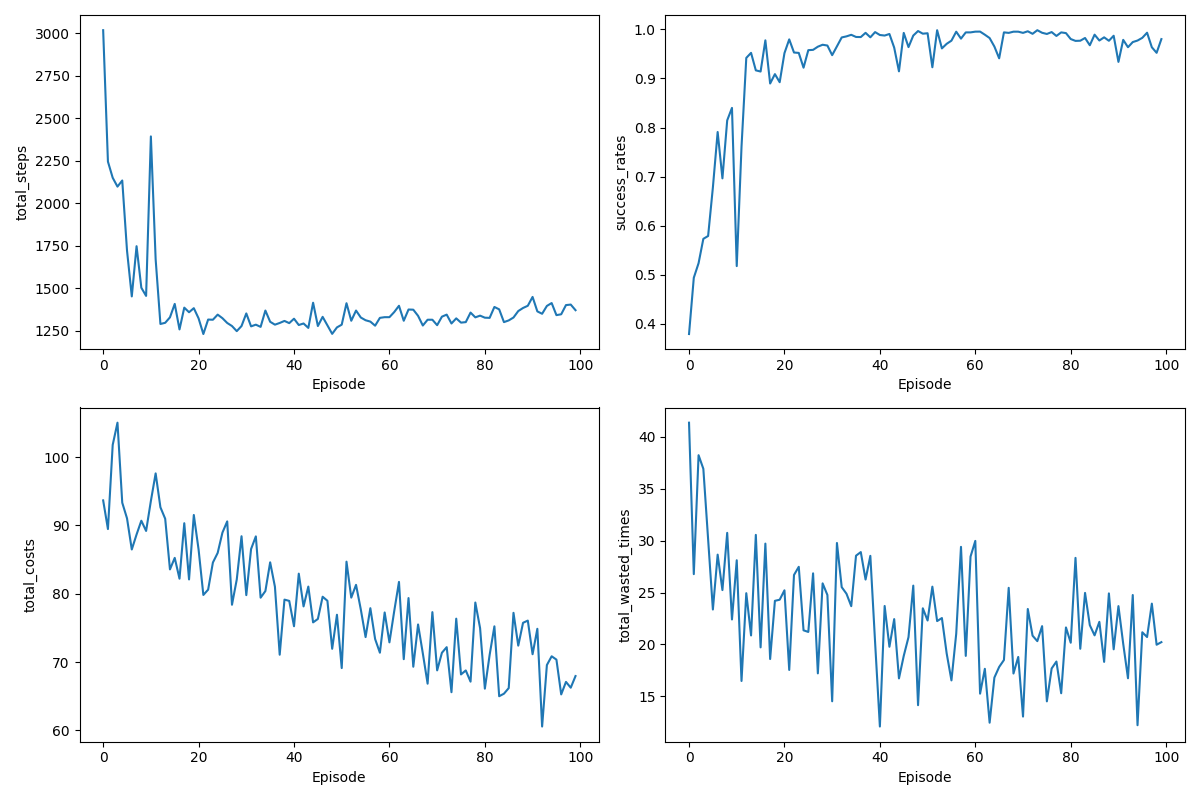
\includegraphics[height=0.7\textheight]{pics/train.png}
        \caption{训练过程中调度总数、调度成功率、总开销、总浪费时间的变化}
    \end{figure}

\end{frame}

\begin{frame}{调度算法评估}

    \begin{figure}
        \centering
        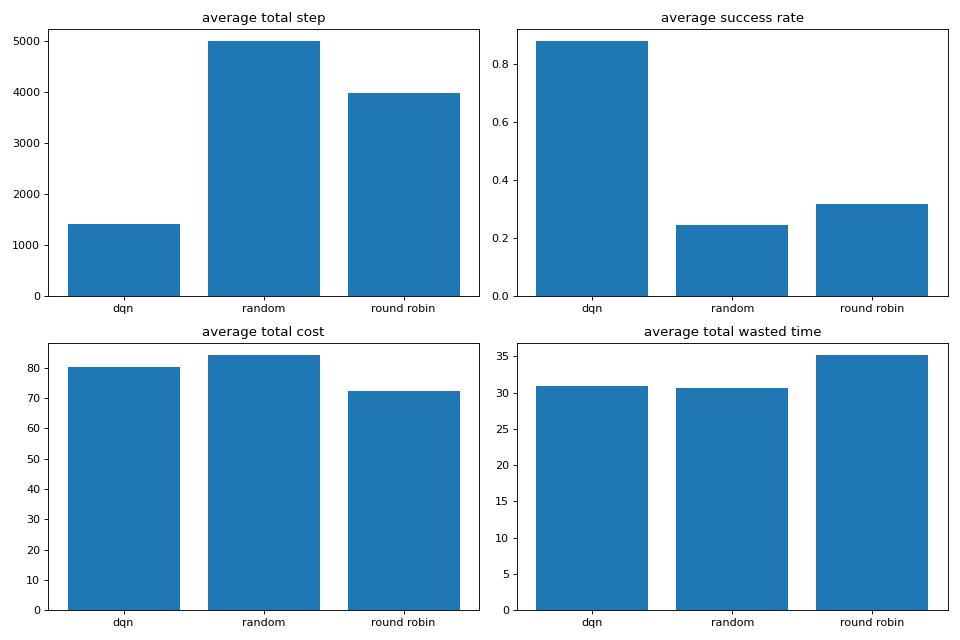
\includegraphics[height=0.7\textheight]{pics/evaluate.png}
        \caption{DQN、Random、Round-Robin三种调度算法的表现}
    \end{figure}

    Earliest算法无法完成该数学模型下的调度任务.

\end{frame}


\section{问题与展望}

\begin{frame}{问题一: 时间指标}

    在任务调度流程中, 记录了每次调度任务的提交时刻 $t_s$, 开始时刻 $t^b$ 和结束时刻 $t^e$.
    应当如何使用这些时间数据更好地比较不同调度算法的性能?

    目前想到的方法:
    \begin{enumerate}
        \item 比较平均每次任务调度的响应时间 $t^e - t_s$
        \item 比较平均每次任务调度的相应比 $t^e - t_s / t^e - t^b$
        \item 比较平均每个任务从第一次提交到最终全部完成的时间
    \end{enumerate}

\end{frame}

\begin{frame}{问题二: 调度成功率}

    目前DRL调度算法的成功率不能达到 100\%. 为了保证调度流程能够正常进行, 在DRL调度失败时使用Round-Robin调度算法, 将任务分配到可以执行的实例上.

    是否有可行的办法使DRL调度算法的成功率稳定在 100\%?

    \begin{enumerate}
        \item 应用DQN的全部高级技巧: 优先经验回放、双Q学习、对决网络和噪声网络
        \item 增加训练轮数
        \item \dots
    \end{enumerate}

\end{frame}


\section{参考文献}

\begin{frame}{参考文献}

    \bibliographystyle{plain}
    \bibliography{reference/ref}
    \nocite{downeyParallelWorkloadModel1998}
    \nocite{leslieExploitingPerformanceCost2013}

\end{frame}


\end{document}
